%!TEX root = main.tex

\section{Performance Evaluation}

\label{sec:simulation}

In this section, we study the performance of the proposed mechanism using ndnSim\cite{ndnsimnet, ndnsim}.

Our evaluation includes four parts. In the first part we discuss the influence of $\alpha$ and $\beta$ in Eq.~\ref{eq:updated_rt5} to system stability. In the second part we evaluate the flow number estimating process, which we propose in Eq.~\ref{eq:flownum}. In the third part, we evaluate the ECN-based Interest sending(ECN-based) mechanism using the bottleneck network topology. At last we join the Smart forwarding with ECN-based(SECN) and evaluate SECN using the mesh network topology. The evaluation results show the flow number can be estimated accurately. Compared with ICP and ICP-shape, ECN-based mechanism performs better in link utilization, packets dropping and flow complete time. The SECN has better TFCT(Total Flow Complete Time) compared with adaptive forwarding mechanism.

\subsection{Network Setup}
Fig.~\ref{mesh-topology} and Fig.~\ref{bottleneck-topology} show the two network topologies we use in the simulation. One is bottleneck topology and the other one is mesh topology. In both network topologies, there are many consumers who send Interest into network and retrieve the corresponding Data from the producer. The number of consumers varies from 1 to 100. In the mesh network, consumers can get Data from three paths and each path's bottleneck bandwidth is different. Each link's capacity varies from 30~Mbps to 200~Mbps and the propagation delay of each hop is 10~ms. The buffer in each node is equal to the production of bandwidth and delay. In the following, the bandwidth refers to the bottleneck's bandwidth.

\begin{figure}[t]
\centering
\includegraphics[width=2.5in]{bottleneck-topology.pdf}
\caption{Bottleneck topology using in simulation.}
\label{bottleneck-topology}
\end{figure}

\subsection{Stability analysis}
To choose suitable $\alpha$ and $\beta$ that make the system stable, we test under what $\alpha$ and $\beta$, the flow number can be estimated accurately. Once the flow number of the network can be accurately estimated, the Interest sending rate $R_{r}(t)$ can also be estimated accurately, then the system enters stable stage. So we choose the accuracy of estimating flow number as the stability metrics.

At the beginning, there are 10 flows in the network, and we test whether the flow number can accurately be estimated under different value of $\alpha$ and $\beta$. Fig.~\ref{fig-ab} shows that under such values the flow number can be accurately estimated. Fig.~\ref{fig-abwrong} shows that under these values the estimated flow number change greatly, which means that the system is not stable. From Fig.~\ref{fig-ab}, we can find (0.2,1.5) is the most suitable value to estimate the flow number. Under this value, we test whether the system is still stable when the system changes. We set the number of flows in the network as 5,10,15 and 20 respectively. Fig.~\ref{fig-abflownum} shows that under different situations the flow number can also be accurately estimated when $\alpha=0.2,  \beta=1.5$. That means a fixed value of $\alpha$ and $\beta$ can make the system enter stable stage even when the system's situation changes.

From Fig.~\ref{fig-abwrong}, we find that when $\alpha$ is close to 0.5, the system becomes unstable, and when it gets larger, the system becomes even more unstable. This can be explained as follows. Large $\alpha$ makes the system react too radically to increase $R_{r}(t)$ when $(C-S(t))>0$ or decrease $R_{r}(t)$ when $(C-S(t))<0$. Radical reaction will make the system difficult to converge. From Fig.~\ref{fig-ab}, we find that when $\alpha < 0.2$, the system will take longer time to accurately estimate the flow number. It is because small $\alpha$ makes the system increase or decrease $R_{r}(t)$ conservatively, and that will result in longer time to convergence. When $\beta$ is smaller than 1.5, although the system can be stable, the estimated flow number is not accurate compared with $\beta = 1.5$. It is because small $\beta$ can not drain the packets in the queue quickly enough. And that will result in inaccurate $R_{r}(t)$ and flow number.

The key point of the stability analysis is that, for $\alpha$ and $\beta$ we can choose a fixed value to make the system stable. Even when the system changes, such as the flow number, RTT and bandwidth, the fit value can also make the system keep stable. Although now we can not prove the best value by theory, it is possible to choose a stable value. In our simulation, we set $\alpha = 0.2$ and $\beta = 1.5$, according the analysis above.

\begin{figure}[t]
\centering
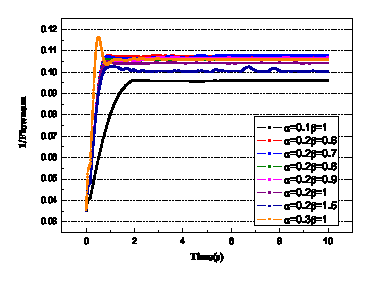
\includegraphics[width=2.5in]{ab-pic-cut.eps}
\caption{Under such $\alpha$ and $\beta$ the flow number can be accurately estimated.}
\label{fig-ab}
\end{figure}

\begin{figure}[t]
\centering
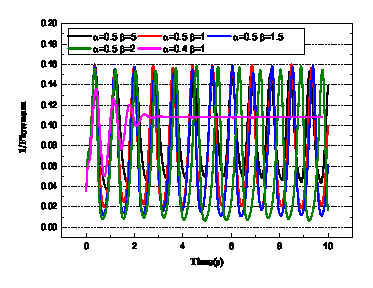
\includegraphics[width=2.5in]{abwrong-pic-cut.eps}
\caption{Under such $\alpha$ and $\beta$ the flow number can not be accurately estimated.}
\label{fig-abwrong}
\end{figure}

\begin{figure}[t]
\centering
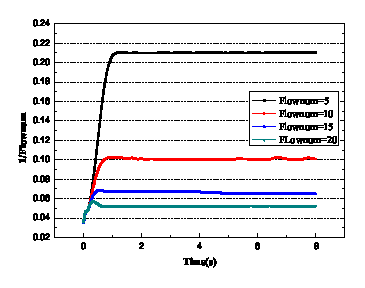
\includegraphics[width=2.5in]{abflownum-pic-cut.eps}
\caption{Stable $\alpha$ and $\beta$ can make the network stable even when network situation changes.}
\label{fig-abflownum}
\end{figure}

\subsection{The estimated flow number}

 Following Eq.~\ref{eq:flownum}, the flow number of the link can be estimated by the rate of this link. The size of Data can be estimated as the average size of the Data that goes through. Under the bottleneck network topology, at t=0, 10 flows start. At t=10 another 10 flows start. And at t=20, 10 flows finish, there are only 10 flows left. From Fig.~\ref{fig-flownum} we can see that the flow number can be accurately estimated. Even when the flow number changes, the estimation can also converge.

\begin{figure}[t]
\centering
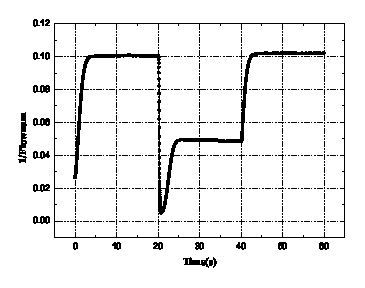
\includegraphics[width=2.5in]{flownum-pic-cut.eps}
\caption{The accuracy of estimation of flow number.}
\label{fig-flownum}
\end{figure}

\subsection{The performance of ECN-based Interest sending rate mechanism}

We use bottleneck topology to assess the ECN-based mechanism. ICP is a TCP-style Interest control protocol in NDN. The Interest sending window is passively changed according the RTT and loss of Data, following the AIMD principle\cite{ICP}. ICP-shape also follows the AIMD principle but it discards the Interest instead of Data when the routers sense congestion\cite{improveshape}. ICP-shape also sends NACK back to receiver if an Interest is shaped. NACK is a feedback information used to inform that the Interest has been discarded or there's no Data corresponding to the Interest. The consumer should retransmit the same Interest when it receives a NACK. As Fig.~\ref{fig-linkuti} shows, ICP and ICP-shape waste bandwidth because of the slow start and AIMD principle. The link utilization of ICP and ICP-shape is between 80\%-90\%. In contrast, even when the bottleneck link's bandwidth changes, the bandwidth utilization of ECN-based always closes to 100\%.

\begin{figure}[t]
	\centering
	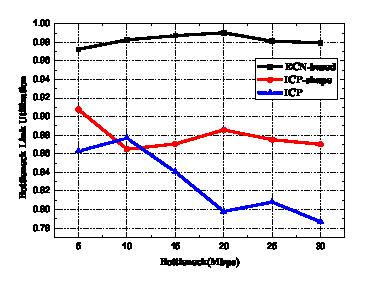
\includegraphics[width=2.5in]{utilization-pic-cut.eps}
	\caption{The bottleneck's link utilization compared with ICP and ICP-shape when change the bottleneck bandwidth.}
	\label{fig-linkuti}
\end{figure}

Because the ECN-based makes sure that the rate can't exceed the bandwidth, almost no packet (no matter Interest or Data) drops in ECN-based mechanism, as the Fig.~\ref{fig-drop} shows. ICP uses timeout as the signal to inform congestion, and timeout is caused by dropping Data. In ICP, once the link become congested, the only solution is to drop Data, so the number of dropped Data is very large. The ICP-shape shapes Interest before congestion happens, so it can reduce the number of Data needed to be dropped because of congestion. But as the delay of sending back and the difficulty of estimating the congestion, there are still some dropped Data.

\begin{figure}[t]
	\centering
	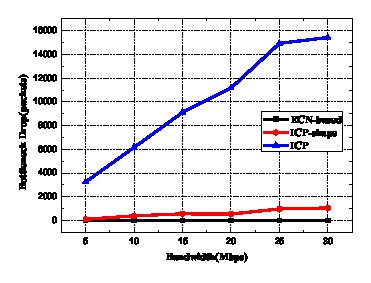
\includegraphics[width=2.5in]{drop-pic-cut.eps}
	\caption{The number of dropping packets in bottleneck compared with ICP and ICP-shape when change the bottleneck bandwidth.}
	\label{fig-drop}
\end{figure}

As Eq.~\ref{eq:updated_rt5} shows, the packets in the queue should be drained. This principle makes sure that in ECN-based, the number of packets in the queue are always close to 0, as shown in Fig.~\ref{fig-queue}.In ICP, to use the bandwidth effectively, the receivers always try to enlarge the Interest window until the Data fills up the queue and the Data is dropped, so the number of packets in the queue is largest compared with other two mechanisms. In ICP-shape, the router can shape Interest when it senses that congestion happens. So in ICP-shape, the number of queue size is less than ICP, as shown in Fig.~\ref{fig-queue}.

\begin{figure}[t]
	\centering
	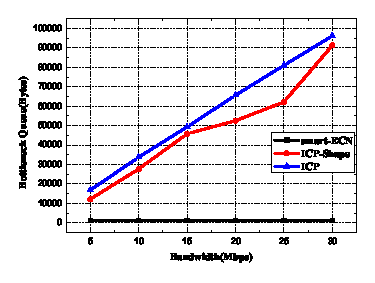
\includegraphics[width=2.5in]{queu-pic-cut.eps}
	\caption{The queuing packets in bottleneck compared with ICP and ICP-shape when change the bottleneck bandwidth.}
	\label{fig-queue}
\end{figure}

Fig.~\ref{fig-fct} shows the FCT(Flow Complete Time) of different flows. FCT in NDN is defined as the time from when receiver sends the first Interest until the receiver receives the last Data of the flow. The ECN-based mechanism's link utilization is much higher than ICP. ECN-based mechanism fairly distributes bandwidth resource to all the flows, so even the short flow can get fair bandwidth resource. No matter flows are short or long, ECN-based'FCT is much better than ICP.

\begin{figure}[t]
	\centering
	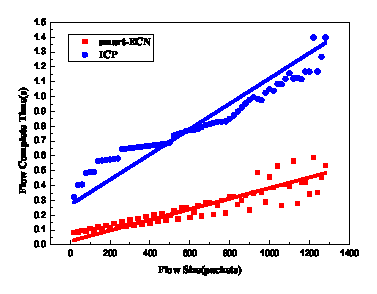
\includegraphics[width=2.5in]{fct-cut.eps}
	\caption{ECN-based's flow complete time compared with ICP.}
	\label{fig-fct}
\end{figure}

\subsection{Flow complete time compared with ICP}

We demonstrate the effectiveness of SECN(Smart forwarding with ECN-based) using mesh network topology ,as shown in Fig.~\ref{mesh-topology}. As Fig.~\ref{fig-tfct} shows, under different total bandwidth, the SECN's TFCT is much better than non-adaptive mechanism. As smart adaptive forwarding mechanism can choose the best path on the network-wide view, it's total flow complete time is even better than adaptive mechanism. The total bottleneck bandwidth refers to the sum of bottleneck bandwidth on all the available paths. Using the forwarding-assistance and route information, as shown in Fig.~\ref{fig-assistant-information}, the smart adaptive forwarding mechanism can choose the network-wide best path. The non-adaptive mechanism chooses the path by the route information, similar with TCP/IP. The non-adaptive mechanism can not change the forwarding interface according to the network condition. The adaptive mechanism chooses the best forwarding interface just by the next hop's link information. As the next hop link information can not reflect the whole path's information, the adaptive mechanism sometimes chooses a path whose later link is shared by far more flows.

\begin{figure}[t]
\centering
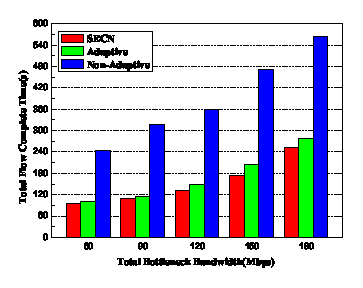
\includegraphics[width=2.5in]{adaptive-pic-cut.eps}
\caption{Total flow complete time compared with other two forwarding mechanisms.}
\label{fig-tfct}
\end{figure}

